\section{Отслеживание контакта роликов при движении омни-колеса}

Чтобы задать уравнение (2), выражающее условие контактирования двух поверхностей, необходимо:
1) найти радиусы-векторы ближайших точек твердых тел (общая нормаль)
2) записать условия равенства проекций скоростей этих точек на общую нормаль

Помимо этого, необходимо вычислить касательную составляющую скорости точки одного тела относительно другого для задания модели касательной составляющей реакции в случае неидеальных связей.


Для наглядности мы ограничиваемся рассмотрением омни-колес, оснащенных четырьмя роликами.  (Рис.~\ref{OmniWheel}).

\begin{figure}[htb]
\centering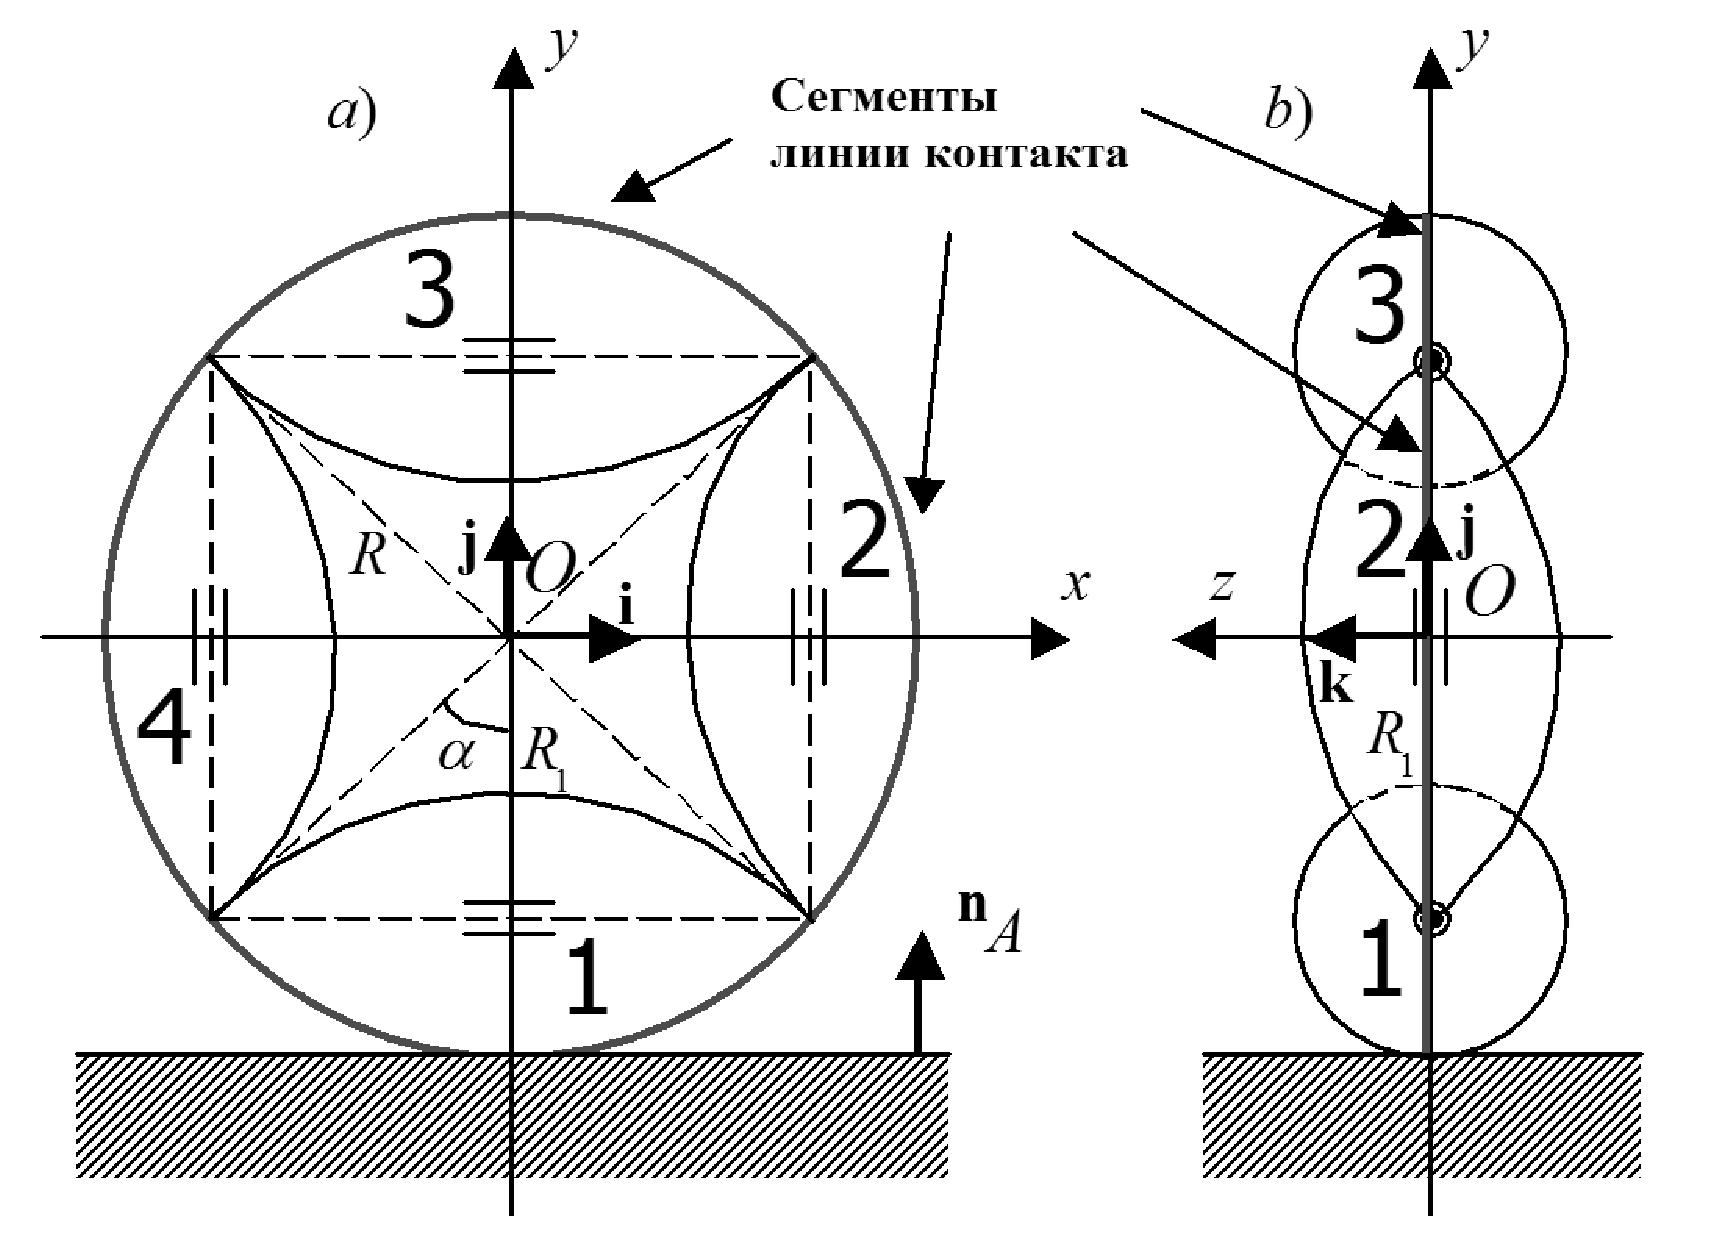
\includegraphics[width=13cm]{content/parts/3_friction/nd/OmniWheel.eps}
\caption{Омни-колесо в вертикальном положении: a) вид сбоку; b) вид спереди.}
\label{OmniWheel}
\end{figure}


%Так что в результате переключение контактов между роликами омни-колеса не приведет к нарушению регулярности движения в силу причин ударного характера. Заметим еще раз, что все описанное будет справедливо, если колесо все время остается в вертикальном положении.

% На следующем уровне сборки модели несколько колес соединяются с подвижной 
% платформой экипажа при помощи шарнирных связей. В нашем случае количество колес 
% может быть три или более (в зависимости от конструкции экипажа и модели 
% контактирования ролика с полом). На платформе они могут образовывать самые 
% разные конфигурации. В конкретном примере Рис.~\ref{Vehicle} имеется три 
% колеса, образующие равносторонний треугольник в горизонтальной плоскости $zx$. 
% Ось $y$ здесь предполагается вертикальной.

% \begin{figure}[htb]
% \centering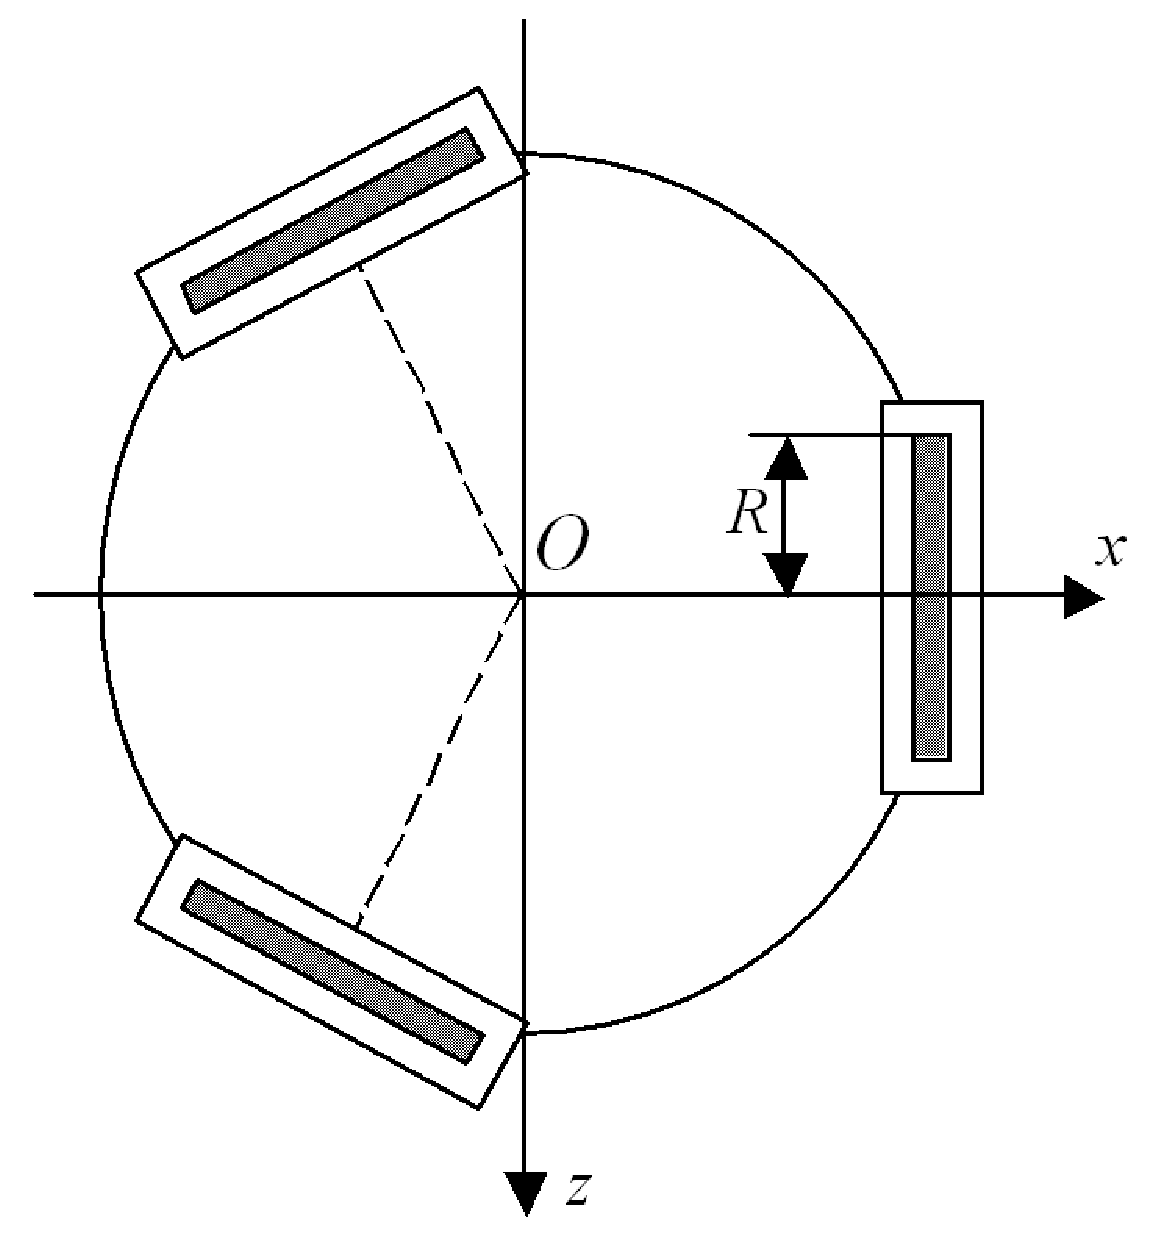
\includegraphics[width=9cm]{content/parts/3_friction/nd/Vehicle.eps}
% \caption{Трехколесный экипаж. Вид сверху.}
% \label{Vehicle}
% \end{figure}

% \section{Модель динамики отдельного ролика.\ }
\label{sec3}
Для начала составим формулы, задающие геометрическую одностороннюю связь контакта одного неусеченного ролика и плоскости. Введем оси $Oxyz$, жестко связанные с роликом, следующим образом: ...
Напомним, что ролик ограничен поверхностью вращения дуги окружности радиуса $l$ вокруг ее хорды, так что  уравнение поверхности имеет вид (см. фиг.~\ref{Roller}):
\begin{equation}
x^2+\left(\sqrt{y^2+z^2}+R_1\right)^2=R^2,
\label{3_1}
\end{equation}
ОБОЗНАЧЕНИЯ!!!
где $R$ --- радиус омни-колеса, $R_1=R\cos{\alpha }$ --- расстояние от центра
ролика до центра колеса, $\alpha =\pi /n$ --- половина центрального угла, под
которым ролик виден из центра колеса, $n$ --- количество роликов на колесе.

\begin{figure}[htb]
\centering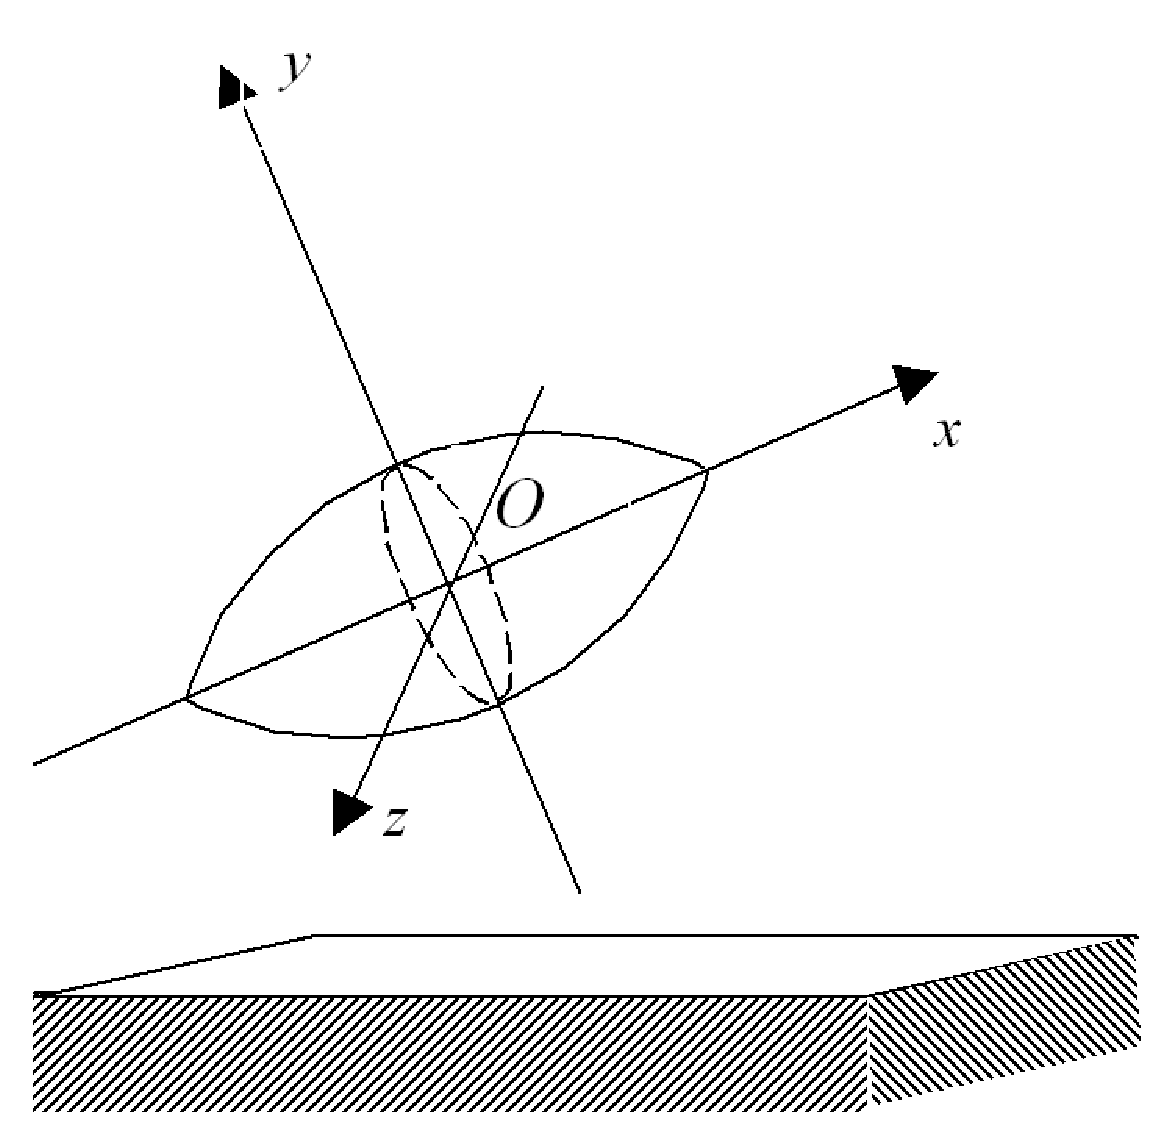
\includegraphics[width=10cm]{content/parts/3_friction/nd/Roller.eps}
\caption{Ролик над горизонтальной плоскостью. Вид сбоку.}
\label{Roller}
\end{figure}

\cite{Kosenko2007}\cite{Kosenko2006}

% Динамика поступательно-вращательного движения реализуется так, как это описано в, в виде уравнений Ньютона -- Эйлера. Причем для моделирования вращательного движения твердого тела используется алгебра кватернионов~\cite{KosenkoQuaternionRus,Kosenko1998}.

Сказать, что здесь можно острие!
И что мы этим воспользовались, но не только, а еще и усеченные тоже.
    МЫСЛЬ СКОЛЬЗИТЬ МОЖНО !.

Заметим, что эта поверхность имеет  в 
точках $x=\pm R\sin\alpha $ особенность, что в численных алгоритмах обычно приводит к аварийному завершению вычислительного процесса моделирования.

В нашей задаче положение спасает специфика конфигурации, обеспечивающей 
постоянство вертикального расположения омни-колес, так что касательная плоскость к поверхности ролика определена при любух значениях координат. При этом условии можно
указать явную формулу, позволяющую вычислить ближайшую к плоскости точку $P_B$
ролика (Рис.~\ref{ContactScheme}). Этой точке всегда <<противостоит>> её 
вертикальная проекция $P_A$ на плоскость (Рис.~\ref{ContactScheme}).

\begin{figure}[htb]
\centering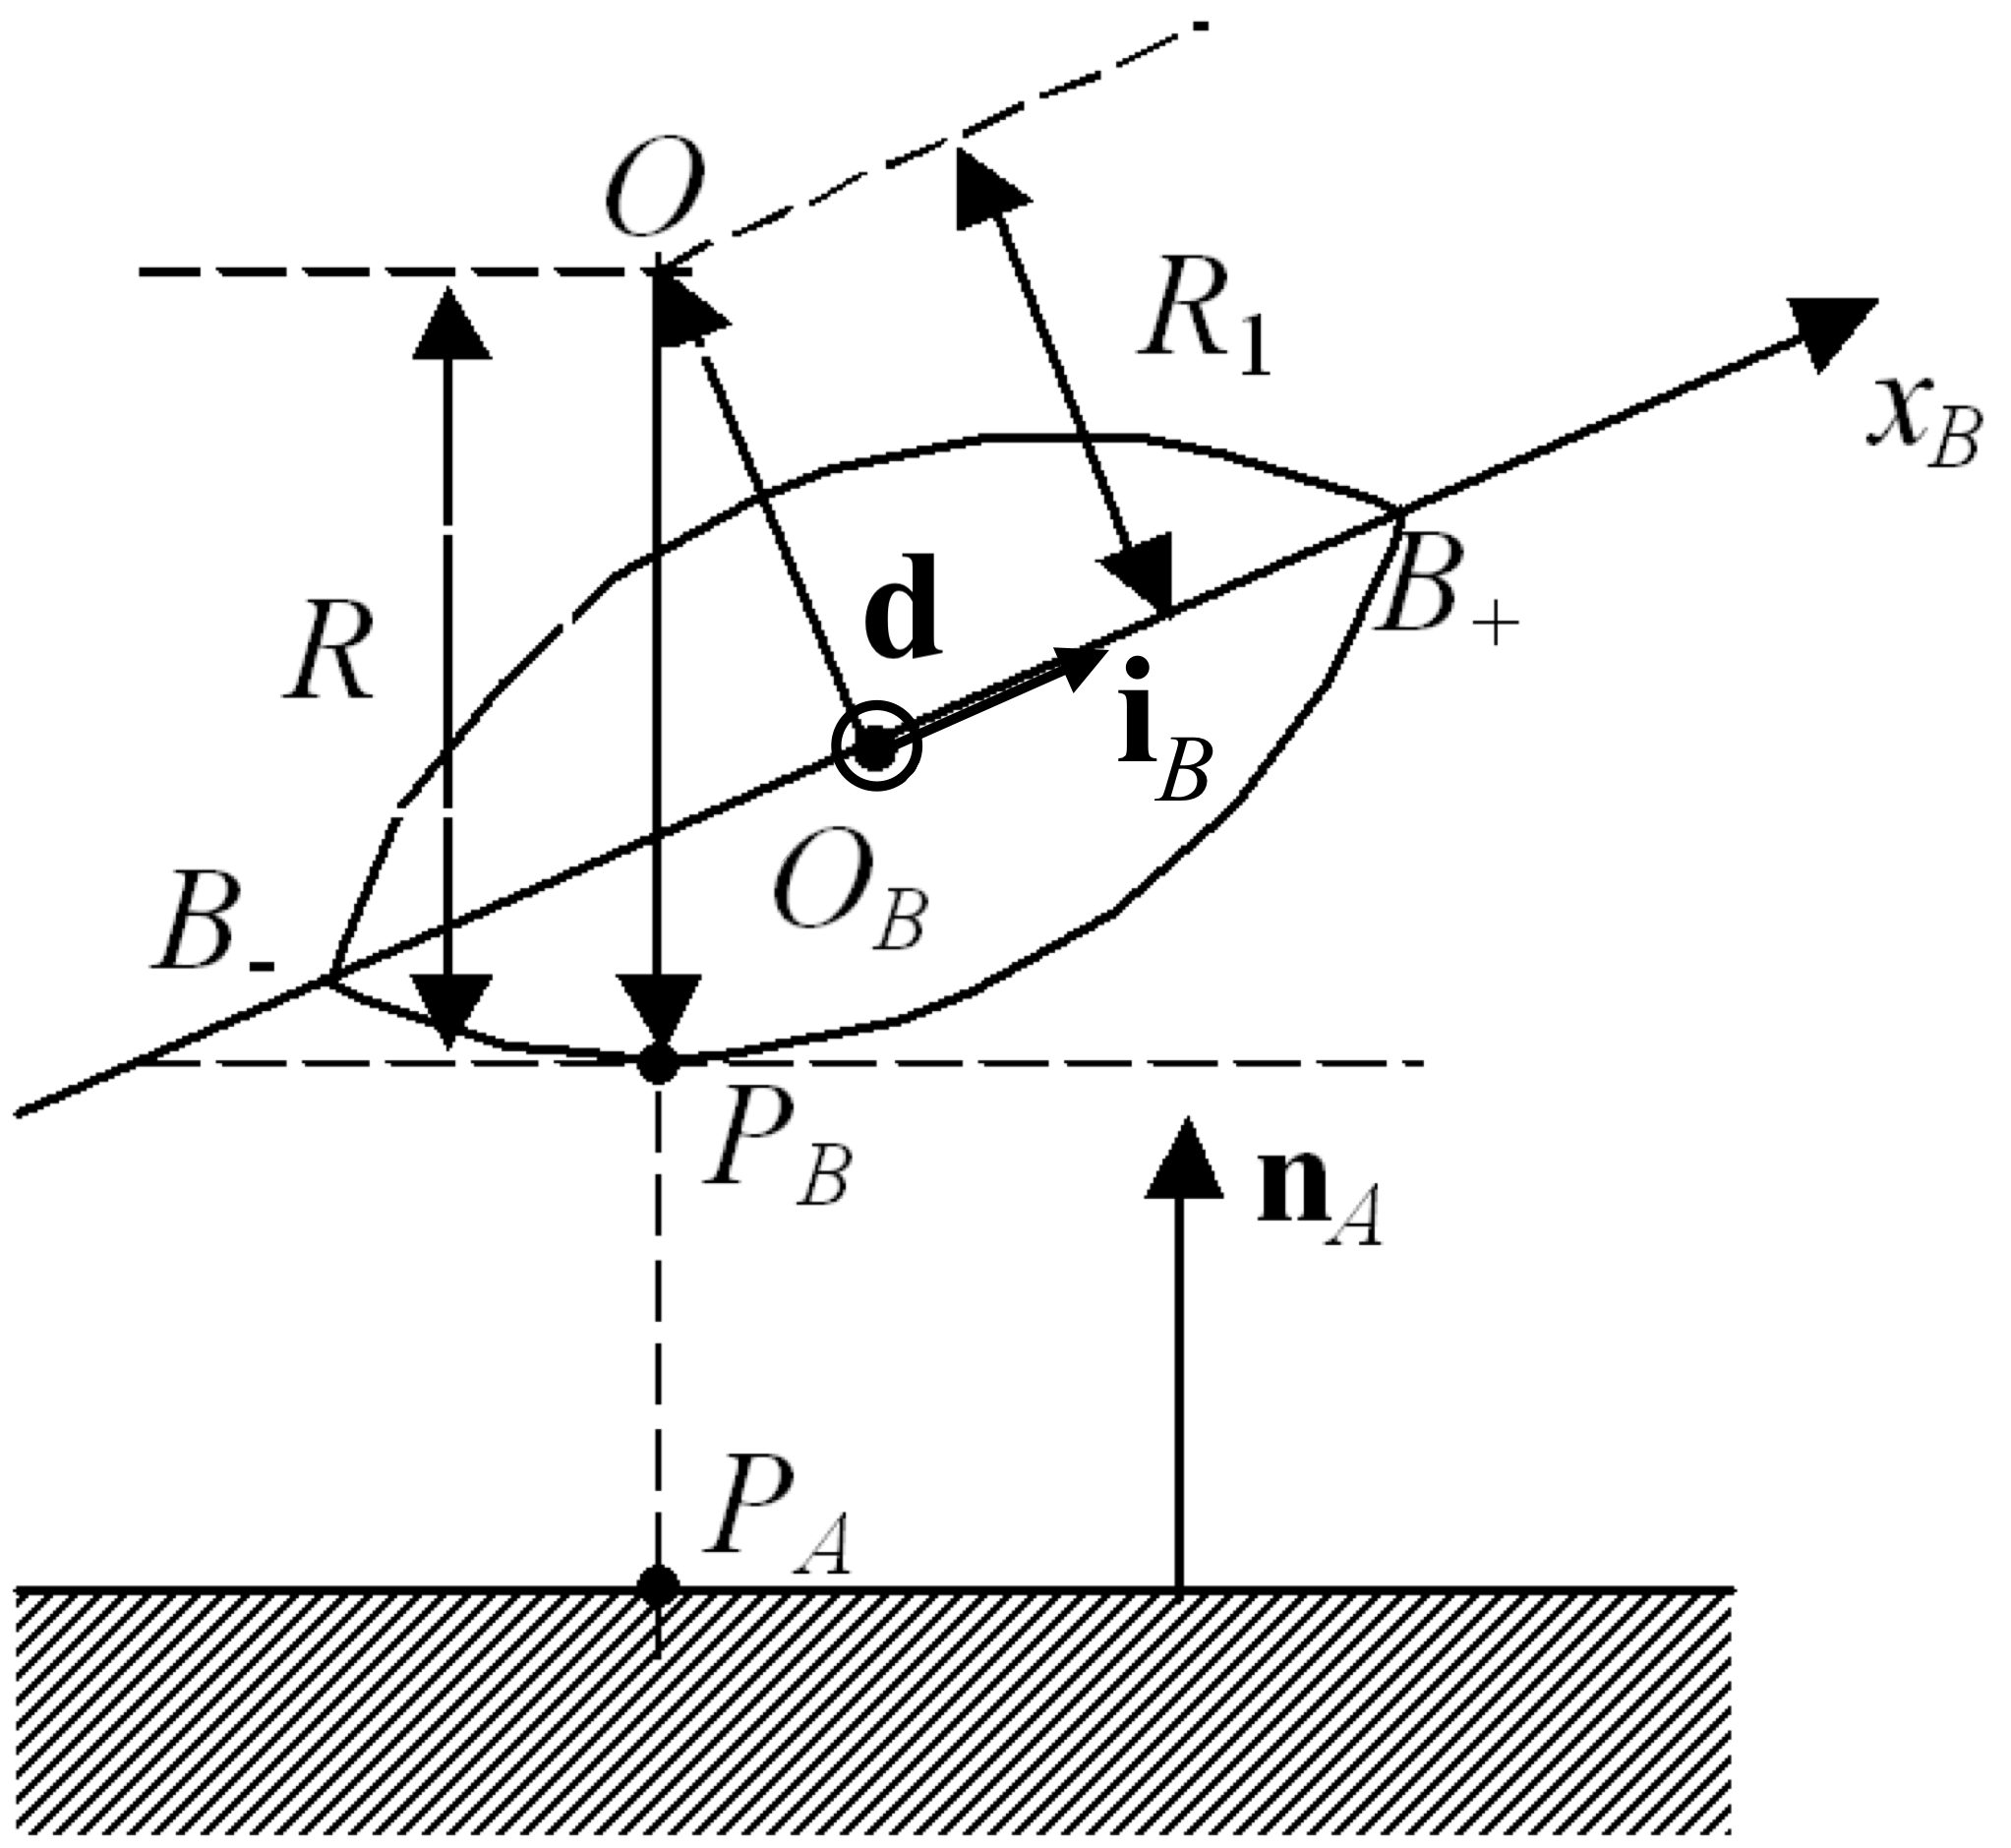
\includegraphics[width=8cm]{content/parts/3_friction/nd/RollerSection_d_ib.png}
\caption{Схема отслеживания контакта: вид сбоку отдельного ролика.}
\label{ContactScheme}
\end{figure}

!!!!!!!!!!!!!!В последующем тексте:
меняем обозначения на принятые ранее, убираем произведение матриц.

Обозначим ${\bf i}$ --- орт оси ролика,
${\bf r}_B$ ---
радиус-вектор геометрического центра ролика в текущий момент времени и 
${\bf \gamma}$ --- орт нормали к плоскости,  в нашей задаче являющийся единичным вектором восходящей вертикали. 
%Плоскость условно обозначается нами телом с индексом $A$, ролик --- $B$. 
Введем орт ${\bf d}$ --- горизонтальный орт, перпендикулярный плоскости колеса
$$
{\bf d}=\dfrac{{\bf i}\times {\bf \gamma}}
              {\left| {\bf i}\times {\bf \gamma}\right|}.
$$
Пусть $O$ --- центр окружности, вращением дуги которой образована поверхность ролика(Рис.~\ref{ContactScheme}). (Заметим, что эта же точка является центром омни-колеса)  
Тогда, очевидно, отрезок $\overrightarrow{O_BO}$, расположенный в вертикальной
плоскости, будет иметь длину $R_1$ и задаваться формулой
$$
\overrightarrow{O_BO}=R_1{\bf d}\times {\bf i}_B.
$$
 Так что самая нижняя точка $P_B$ внешней 
поверхности ролика будет задаваться по формуле
\begin{equation}
{\bf r}_{P_B}={\bf r}_B+R_1{\bf d}\times T_B{\bf i}_B-R{\bf n}_A,
\label{3_2_0}
\end{equation}
поскольку точка $P_B$ лежит на упоминавшейся выше окружности на общей вертикали 
с точкой $O$. 

%Для вычисления положения точки $P_A$ нужно вторую координату 
%вектора ${\bf r}_{P_B}$ положить равной нулю
%\begin{equation}
%{\bf r}_{P_A}=\left( x_{P_B},0,z_{P_B}\right) ^T.
%\label{3_2_1}
%\end{equation}

Вся описанная выше вычислительная процедура будет справедлива только, если 
вектор $T_B{\bf i}_B$ имеет направление, ограниченное по вертикали углами
$\pm\alpha $. 
Если соответствующий угол превышает значение $\alpha$, то 
следует положить $P_B=B_{-}$, где $B_{-}$ --- левая концевая точка ролика. Если
же этот угол меньше величины $-\alpha $, нужно положить $P_B=B_{+}$, где 
$B_{+}$ --- правая концевая точка ролика.

В конечном итоге условие контактирования ролика и плоскости можно записать в 
виде
\begin{equation}
\left| T_B{\bf i}_B\cdot {\bf n}_A\right|\le\sin\alpha .
\label{3_2}
\end{equation}
Это условие, однако, позволяет из всего множества роликов колеса выделить 
нижний (контактирующий) и верхний. Чтобы отбросить случай последнего ролика
можно к последнему условию присоединить также требование 
\begin{equation}
y_B<R,
\label{3_3}
\end{equation}
где $y_B$ --- высота центра ролика относительно инерциальной системы координат.

Таким образом, конъюнкция условий (\ref{3_2}) и (\ref{3_3}) означает наличие
контакта. В противном случае, при отсутствии контакта, нормальная реакция 
отсутствует. С другой стороны, реализация контакта 
геометрически означает выполнение скалярного условия 
\begin{equation}
y_{P_B}=0,
\label{3_4}
\end{equation}
а его отсутствие --- также скалярного (альтернативного) условия
$$
F_n=0,
$$
где $F_n$ --- нормальная составляющая реакции (в данном случае отсутствующей) 
приложенной в точке $P_B$.

% \begin{figure}[htb]
% \centerline{
% 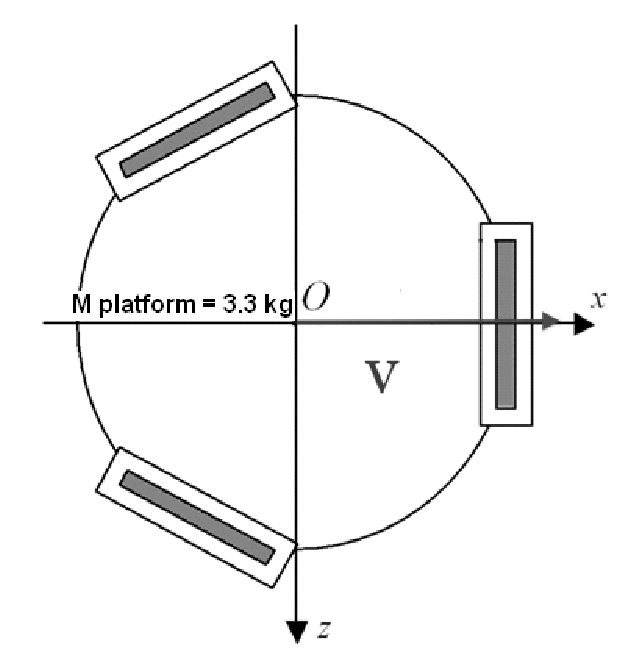
\includegraphics[width=7cm]{content/parts/3_friction/nd/Translat.eps}
% 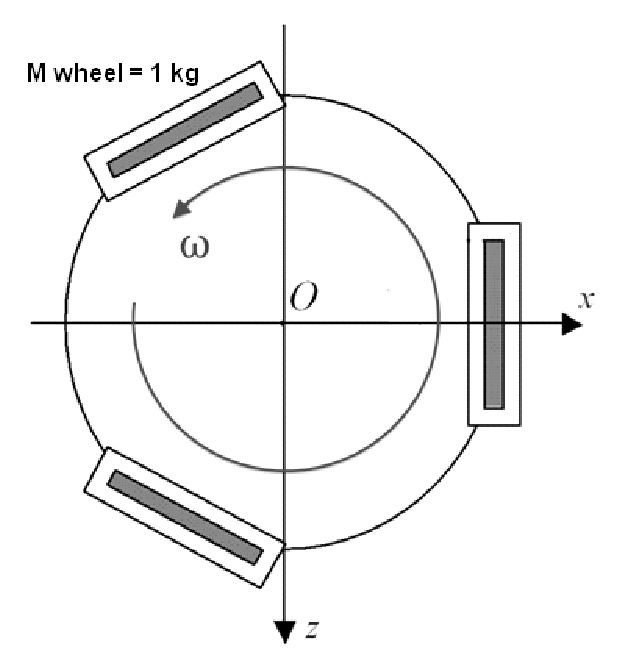
\includegraphics[width=7cm]{content/parts/3_friction/nd/Rotat.eps}
% }
% \caption{Типы движения при верификации модели.}
% \label{TypesOfMotion}
% \end{figure}

Вычислительная практика показала, что уравнения контакта в форме (\ref{3_4})
стабильно приводит к аварийному завершению процесса симуляции динамической 
модели ролика. Аналогичный результат получается, если в качестве уравнения 
контактирования использовать уравнение вида 
$$
v_n=0,
$$
где $v_n$ -- нормальная составляющая скорости точки контактирования, лежащей
на теле $B$, относительно тела $A$ (горизонтальной плоскости). И только 
уравнение вида
$$
\dot{v}_n=0
$$
приводит к требуемому результату -- корректной работе объекта контактирования
(реализованного в данном случае на языке Modelica~\cite{Fritzson}) в процессе 
симуляции модели. Вся реализация процесса контактирования 
выполнена в предположении точечного <<твердого>> контакта твердых тел без 
какой-либо податливости.

Колеса, собранные в экипаж, с неизбежностью будут сохранять вертикальное 
положение. Поэтому упрощенный алгоритм отслеживания контакта, описанный выше,
всегда будет работать правильно.

Поскольку ролики, вообще говоря, входят и выхоядят из состояния контакта с опорной плоскостью, то и силы трения и нормальные реакции приложены к роликам не во все время движения, и требуется указать кинематические условия, при которых имеется контакт.

Итак, ролик находится в контакте, если только если $\vec{s} \cdot \vec{e}_z < \cos\ddfrac{\pi}{n} $ и $ z_C < l $. В противном случае со стороны опорной плоскости к ролику не приложены силы. В случае контакта, сперва найдем координаты и скорость точки ролика, находящейся в данный момент на опорной плоскости:

$$ \vec{r}_C = \vec{r}_K + r\vec{s} - l\vec{e}_z + \lambda\vec{k}_1 $$
$$ \lambda = \ddfrac{\left(r\vec{s} - l\vec{e}_z\right)\cdot\vec{k}_2}{ \vec{k}_1\cdot\vec{k}_2} $$
$$ \vec{v}_C = \vec{v}_K + [ \vec{\omega}_{\text{рол}}, \overrightarrow{KC} ] $$

Тогда для определения реакций воспользуемся уравнениями:
$$ \vec{v}_C \cdot \vec{e}_z = 0 $$
$$ \vec{R}_{\text{к}} = \vec{F}_{\text{тр}} + N\vec{e}_z $$
Иначе $ \vec{R}_{\text{к}} = \vec{0} $
